% !TEX root = ../main.tex

\documentclass[../main.tex]{subfiles}

\graphicspath{{\subfix{../images/}}}

\begin{document}

\subsection{Выбор среды разработки и языков программирования}

Разработка кроссплатформенного мобильного приложения предполагает выбор технологии, позволяющей совместить единую бизнес-логику с нативной производительностью на целевых платформах. Для решения данной задачи рассматривались три основных подхода: раздельная нативная разработка (Kotlin для Android, Swift для iOS), гибридные фреймворки (React Native, Flutter) и технология Kotlin Multiplatform (KMP).

При раздельной нативной разработке каждая платформа реализуется независимо. Такой подход обеспечивает максимальную гибкость и полный доступ к платформенным API, однако требует дублирования логики, что увеличивает трудозатраты на сопровождение и повышает риск расхождения функциональности между версиями приложения.

Гибридные фреймворки позволяют использовать единую кодовую базу, но зачастую полагаются на собственный рендеринг интерфейса или на JavaScript-мост, что может ограничивать интеграцию с нативными компонентами и влиять на производительность.

Kotlin Multiplatform предлагает иной компромисс: общий код на языке Kotlin компилируется в нативные бинарные файлы для каждой целевой платформы, а платформенно-специфичные части выделяются через механизм \texttt{expect/actual}. Данный подход позволяет переиспользовать до 90\% кодовой базы при сохранении доступа к нативным API там, где это необходимо.

Сравнительная характеристика рассмотренных подходов представлена в табл.~\ref{tab:crossplatform-compare}.

\aboverulesep=0ex
\belowrulesep=0ex
\begin{small}
\begin{longtable}[t]{
	|>{\raggedright}p{0.22\linewidth} |
	>{\raggedright}p{0.22\linewidth} |
	>{\raggedright}p{0.22\linewidth} |
	>{\raggedright\arraybackslash}p{0.24\linewidth}|
}

\caption{Сравнение подходов к кроссплатформенной разработке мобильных приложений} \label{tab:crossplatform-compare}\\
\midrule
Критерий & Нативная разработка & React Native / Flutter & Kotlin Multiplatform \\
\midrule
\endfirsthead

\caption*{Продолжение табл. \ref{tab:crossplatform-compare}\raggedleft}\\\midrule
Критерий & Нативная разработка & React Native / Flutter & Kotlin Multiplatform \\
\midrule
\endhead

\endfoot
\midrule
\endlastfoot

Переиспользование кода &
Низкое &
Высокое &
Высокое \\
\midrule
Производительность &
Максимальная &
Средняя &
Высокая (нативная компиляция) \\
\midrule
Доступ к платформенным API &
Полный &
Ограниченный &
Полный (через \texttt{actual}) \\
\midrule
Единый язык разработки &
Нет &
Частично (JS/Dart + нативный код) &
Да (Kotlin) \\
\midrule
Зрелость экосистемы &
Высокая &
Высокая &
Растущая \\

\end{longtable}
\end{small}

Для проекта Achi выбран Kotlin Multiplatform в связи с необходимостью поддержки платформ Android, Web (WasmJS) и iOS из единого модуля \texttt{shared} без переписывания бизнес-логики. Язык Kotlin обеспечивает статическую типизацию, поддержку корутин для асинхронных операций и тесную интеграцию с экосистемой JetBrains.

В качестве среды разработки используется Android Studio с плагинами Kotlin Multiplatform и Compose Multiplatform. Сборка проекта осуществляется системой Gradle; версии ключевых компонентов зафиксированы в каталоге зависимостей (\texttt{libs.versions.toml}): Kotlin~2.3.0, Compose Multiplatform~1.10.0, Ktor~3.3.3.

Целевые платформы приложения Achi и их текущий статус приведены в табл.~\ref{tab:platforms}.

\begin{small}
\begin{longtable}[t]{
	|>{\raggedright}p{0.25\linewidth} |
	>{\raggedright}p{0.25\linewidth} |
	>{\raggedright\arraybackslash}p{0.35\linewidth}|
}

\caption{Целевые платформы приложения Achi} \label{tab:platforms}\\
\midrule
Платформа & Статус & Минимальная версия \\
\midrule
\endfirsthead

\caption*{Продолжение табл. \ref{tab:platforms}\raggedleft}\\\midrule
Платформа & Статус & Минимальная версия \\
\midrule
\endhead

\endfoot
\midrule
\endlastfoot

Android & Активно (Stable) & Android~7.0 (API~24) \\
\midrule
Web (WasmJS) & Активно (Beta) & Браузеры с поддержкой WebAssembly \\
\midrule
iOS & Активно (Stable) & iOS~14+ \\

\end{longtable}
\end{small}

\subsection{Выбор сторонних библиотек и инструментов}

Помимо базовой платформы KMP, для реализации приложения Achi используется набор сторонних библиотек, отобранных с учётом совместимости с Kotlin Multiplatform, зрелости и соответствия функциональным требованиям. Обоснование выбора ключевых компонентов приведено в табл.~\ref{tab:tech-stack}.

\aboverulesep=0ex
\belowrulesep=0ex
\begin{small}
\begin{longtable}[t]{
	|>{\raggedright}p{0.22\linewidth} |
	>{\raggedright}p{0.22\linewidth} |
	>{\raggedright\arraybackslash}p{0.46\linewidth}|
}

\caption{Технологический стек приложения Achi} \label{tab:tech-stack}\\
\midrule
Компонент & Технология & Обоснование выбора \\
\midrule
\endfirsthead

\caption*{Продолжение табл. \ref{tab:tech-stack}\raggedleft}\\\midrule
Компонент & Технология & Обоснование выбора \\
\midrule
\endhead

\endfoot
\midrule
\endlastfoot

UI-фреймворк & Compose Multiplatform & Декларативный подход; единый UI-код; Material~3 \\
\midrule
HTTP-клиент & Ktor Client & Нативная поддержка KMP; корутины; модульность \\
\midrule
Навигация & Navigation~3 (\texttt{navigation3-ui}) & Типобезопасная KMP-навигация; сериализация маршрутов \\
\midrule
Генерация API & OpenAPI Generator & Автоматическая генерация клиента из спецификации \\
\midrule
Загрузка изображений & Coil~3 & KMP-совместимость; интеграция с Ktor \\
\midrule
Локальное хранилище & Multiplatform Settings & Сохранение токена авторизации на всех платформах \\
\midrule
Выбор файлов & FileKit & KMP-диалоги выбора изображений при создании паков \\
\midrule
Сериализация & kotlinx.serialization & Интеграция с Ktor и Navigation~3 \\

\end{longtable}
\end{small}

\textbf{Compose Multiplatform} --- декларативный UI-фреймворк, основанный на парадигме реактивного обновления интерфейса при изменении состояния. В отличие от XML-вёрстки Android или SwiftUI для iOS, Compose Multiplatform позволяет описывать пользовательский интерфейс на языке Kotlin и переиспользовать экраны на всех целевых платформах. Для приложения Achi используется дизайн-система Material~3 с поддержкой динамических цветов Material You на Android.

\textbf{Ktor Client} --- асинхронный HTTP-клиент, разработанный JetBrains с первоначальной ориентацией на Kotlin. Ktor поддерживает модульную архитектуру (Content Negotiation, Logging) и предоставляет платформенные движки: OkHttp для Android, CIO для WasmJS. В проекте Achi Ktor используется как транспортный слой для сгенерированных OpenAPI-клиентов.

\textbf{Navigation~3} (\texttt{org.jetbrains.androidx.navigation3:navigation3-ui}) --- новая библиотека навигации для Compose Multiplatform, заменяющая Jetpack Navigation Compose в KMP-проектах. Маршруты реализуют интерфейс \texttt{NavKey} и сериализуются через \texttt{kotlinx.serialization}, что обеспечивает типобезопасность и сохранение стека навигации. Для Achi определены маршруты списка паков, списка достижений, деталей достижения, создания пака, профиля и настроек.

\textbf{OpenAPI Generator} (версия~7.18.0) генерирует Ktor-клиент и модели данных из файла спецификации \texttt{Achi\_openapi.json}. Автоматическая генерация снижает вероятность ошибок при интеграции с REST API и упрощает синхронизацию клиента при изменении серверного контракта. Сгенерированные схемы (\texttt{AchievementSchema}, \texttt{AchievementPackSchema}) преобразуются в доменные модели через функции-мапперы.

\textbf{Coil~3} обеспечивает асинхронную загрузку и кэширование изображений (превью паков и достижений) с использованием Ktor Network Fetcher. \textbf{Multiplatform Settings} применяется для персистентного хранения OAuth2-токена и данных сессии пользователя. \textbf{FileKit} предоставляет кроссплатформенные диалоги выбора файлов при загрузке изображений в процессе создания паков достижений.

Следует отметить ряд ограничений выбранного стека: Compose Multiplatform и Kotlin/Wasm для Web-платформы находятся в стадии активного развития; не все популярные Android- и iOS-библиотеки имеют KMP-аналоги; размер итогового бинарного файла KMP-приложения превышает размер чисто нативного. Указанные факторы учтены при планировании архитектуры: приоритет отдан мобильным платформам (Android и iOS), а Web-версия рассматривается как дополнительный канал распространения.

\subsection{Разработка архитектуры приложения}

Архитектура приложения Achi построена на паттерне MVVM (Model--View--ViewModel) с дополнительным слоем Repository и ручным контейнером внедрения зависимостей. Данное решение обеспечивает разделение ответственности между слоями, тестируемость компонентов и совместимость с реактивной моделью Compose.

Структура слоёв приложения представлена на рис.~\ref{pic:architecture-layers}.

\begin{figure}[H]
	\begin{center}
		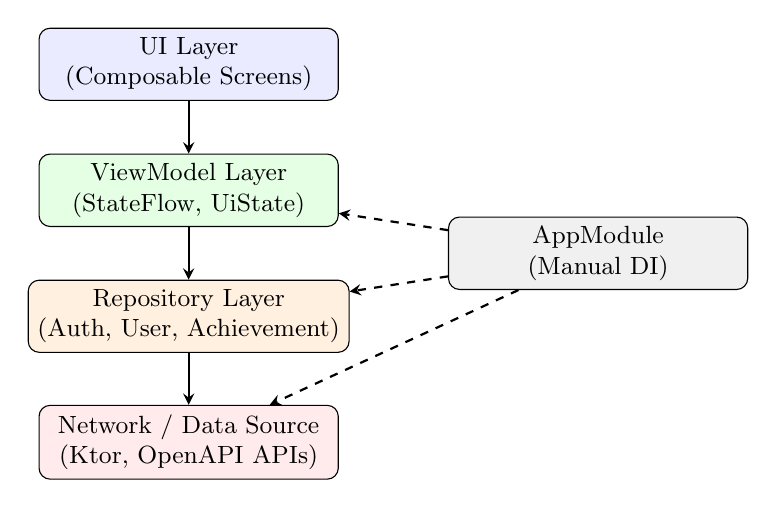
\begin{tikzpicture}[
			box/.style={draw, rounded corners, minimum width=3.8cm, minimum height=0.9cm, align=center, font=\small},
			arrow/.style={->, >=stealth, thick}
		]
			\node[box, fill=blue!8] (ui) at (0, 0) {UI Layer\\(Composable Screens)};
			\node[box, fill=green!10] (vm) at (0, -1.6) {ViewModel Layer\\(StateFlow, UiState)};
			\node[box, fill=orange!12] (repo) at (0, -3.2) {Repository Layer\\(Auth, User, Achievement)};
			\node[box, fill=red!8] (net) at (0, -4.8) {Network / Data Source\\(Ktor, OpenAPI APIs)};
			\node[box, fill=gray!12] (di) at (5.2, -2.4) {AppModule\\(Manual DI)};

			\draw[arrow] (ui) -- (vm);
			\draw[arrow] (vm) -- (repo);
			\draw[arrow] (repo) -- (net);
			\draw[arrow, dashed] (di) -- (vm);
			\draw[arrow, dashed] (di) -- (repo);
			\draw[arrow, dashed] (di) -- (net);
		\end{tikzpicture}
		\captionsetup{justification=centering}
		\caption{Слоистая архитектура приложения Achi}
		\label{pic:architecture-layers}
	\end{center}
\end{figure}

\textbf{Слой представления (View)} содержит Composable-функции экранов, расположенные в пакете \texttt{ui/}. Экраны являются декларативными и не содержат бизнес-логики: они наблюдают состояние ViewModel через \texttt{collectAsState()} и делегируют обработку пользовательских действий методам ViewModel. Навигация между экранами реализована через \texttt{NavDisplay} и \texttt{NavBackStack} библиотеки Navigation~3.

\textbf{Слой ViewModel} располагается рядом с соответствующими экранами и наследует \texttt{androidx.lifecycle.ViewModel}. ViewModel хранит состояние интерфейса в \texttt{MutableStateFlow} и предоставляет неизменяемый \texttt{StateFlow<UiState>} для наблюдения из UI. Для одноразовых событий (сообщения Snackbar, навигация) используются \texttt{Channel} и \texttt{Flow}. Асинхронные операции выполняются в \texttt{viewModelScope} с использованием корутин Kotlin.

\textbf{Слой Repository} инкапсулирует доступ к данным и скрывает детали сетевого взаимодействия от ViewModel. В проекте определены четыре репозитория:
\begin{itemize}[leftmargin=*]
	\item \texttt{AuthRepository} --- аутентификация (логин, регистрация, выход), управление OAuth2-токеном;
	\item \texttt{UserRepository} --- коллекция паков пользователя и синхронизация прогресса;
	\item \texttt{AchievementRepository} --- операции CRUD над достижениями;
	\item \texttt{AchievementPackRepository} --- операции CRUD над паками, загрузка изображений.
\end{itemize}

Репозитории реализуют паттерн Repository: интерфейс определяет контракт, а реализация (\texttt{*Impl}) обращается к сгенерированным API-клиентам. Преобразование сетевых моделей в доменные выполняется функциями-мапперами в пакете \texttt{data/network/}.

\textbf{Внедрение зависимостей} реализовано вручную через класс \texttt{AppModule}, без использования фреймворков Koin или Dagger. Контейнер создаёт API-клиенты (AchievementsApi, PacksApi, AuthenticationApi и др.) и репозитории (ленивая инициализация через \texttt{by lazy}). Экземпляр \texttt{AppModule} создаётся в корневом Composable \texttt{AchiAppNav} и передаётся в провайдер навигации для создания ViewModel.

Выбор Manual DI обусловлен умеренным масштабом проекта: граф зависимостей содержит около десяти компонентов, что делает явное управление зависимостями прозрачным и не требующим дополнительной конфигурации. При росте сложности проекта возможен переход на DI-фреймворк.

Ключевые архитектурные решения приложения Achi:
\begin{enumerate}[leftmargin=*]
	\item единый модуль \texttt{shared} для всего общего кода;
	\item оптимистичные обновления прогресса (UI обновляется немедленно, синхронизация с сервером --- в фоне);
	\item проверка состояния авторизации перед операциями, требующими учётной записи;
	\item локализация через \texttt{composeResources} (английский и русский языки) с абстракцией \texttt{UiText} для сообщений из ViewModel.
\end{enumerate}

\subsection{Проектирование структур данных и интеграции с API}

Предметная область приложения Achi описывается иерархией сущностей: \emph{пак достижений} (\texttt{AchievementPack}) содержит список \emph{достижений} (\texttt{Achievement}), каждое из которых может быть декомпозировано на \emph{шаги} (\texttt{AchievementStep}) с отслеживаемым \emph{прогрессом} (\texttt{StepProgress}).

Доменные модели определены в пакете \texttt{data/model/} и не зависят от сетевого слоя. Серверные модели (\texttt{*Schema}) генерируются OpenAPI Generator и преобразуются в доменные через функции расширения (\texttt{toAchievement()}, \texttt{toAchievementPack()} и др.).

Модель пака достижений представлена классом \texttt{AchievementPack}:

\begin{lstlisting}[caption={Доменная модель пака достижений}, label={lst:achievement-pack}]
data class AchievementPack(
    val id: String,
    val name: String,
    val count: Int,
    val achievementIds: List<String>,
    val previewImageUrl: String? = null,
    val code: String,
    val creatorId: String = ""
)
\end{lstlisting}

Поле \texttt{code} --- уникальный код для добавления пака в коллекцию другого пользователя. Поле \texttt{achievementIds} содержит идентификаторы входящих достижений; полный список объектов \texttt{Achievement} загружается отдельными запросами.

Модель достижения и связанных сущностей:

\begin{lstlisting}[caption={Доменные модели достижения, шага и прогресса}, label={lst:achievement-models}]
data class Achievement(
    val id: String,
    val title: String,
    val shortDescription: String,
    val longDescription: String? = null,
    val steps: List<AchievementStep>,
    val previewImageUrl: String? = null,
    val imageUrl: String? = null,
    val isCompleted: Boolean = false,
    val creatorId: String = ""
)

data class AchievementStep(
    val id: String,
    val description: String,
    val progress: StepProgress = StepProgress(),
)

data class StepProgress(
    val substepsDone: Int = 0,
    val substepsAmount: Int = 1
)
\end{lstlisting}

Модель \texttt{StepProgress} поддерживает инкрементальный прогресс: пользователь может выполнить $N$ из $M$ подшагов (например, «прочитать 3 из 5 глав»). Для достижений без шагов (\texttt{steps.isEmpty()}) используется бинарный флаг \texttt{isCompleted}. Вычисляемые свойства \texttt{progress}, \texttt{isDone} и \texttt{stepsDone} определяют общий прогресс достижения на основе состояния шагов.

Связь доменных моделей с REST API реализована через набор сгенерированных клиентов, перечисленных в табл.~\ref{tab:api-clients}.

\begin{small}
\begin{longtable}[t]{
	|>{\raggedright}p{0.28\linewidth} |
	>{\raggedright}p{0.32\linewidth} |
	>{\raggedright\arraybackslash}p{0.30\linewidth}|
}

\caption{API-клиенты приложения Achi и их назначение} \label{tab:api-clients}\\
\midrule
API-клиент & Основные операции & Доменные сущности \\
\midrule
\endfirsthead

\caption*{Продолжение табл. \ref{tab:api-clients}\raggedleft}\\\midrule
API-клиент & Основные операции & Доменные сущности \\
\midrule
\endhead

\endfoot
\midrule
\endlastfoot

\texttt{AuthenticationApi} & Получение OAuth2-токена & --- \\
\midrule
\texttt{UsersApi} & Регистрация пользователя & --- \\
\midrule
\texttt{PacksApi} & CRUD паков, поиск по коду & \texttt{AchievementPack} \\
\midrule
\texttt{AchievementsApi} & CRUD достижений & \texttt{Achievement} \\
\midrule
\texttt{UserCollectionApi} & Коллекция паков пользователя & \texttt{AchievementPack} \\
\midrule
\texttt{UserProgressApi} & Синхронизация прогресса шагов & \texttt{StepProgress} \\
\midrule
\texttt{UploadApi} & Загрузка изображений & --- \\

\end{longtable}
\end{small}

Базовый URL сервера задаётся в объекте \texttt{ApiConfig} и может изменяться в режиме отладки через панель Debug Panel. Токен авторизации инжектируется во все API-клиенты через \texttt{AuthRepository} при успешном входе и удаляется при выходе.

Состояние аутентификации описывается data class \texttt{AuthState}, содержащим флаги \texttt{isLoggedIn}, \texttt{username}, \texttt{userId}, \texttt{accessToken} и поля для отображения ошибок. Репозиторий предоставляет \texttt{StateFlow<AuthState>}, на который подписываются ViewModel для адаптации интерфейса (отображение формы входа или данных профиля).

Поток данных при обновлении прогресса шага иллюстрирует интеграцию слоёв:
\begin{enumerate}[leftmargin=*]
	\item пользователь нажимает кнопку увеличения прогресса на экране деталей достижения;
	\item \texttt{AchievementDetailsViewModel} оптимистично обновляет локальное состояние \texttt{UiState};
	\item при наличии активной сессии ViewModel вызывает \texttt{UserRepository.updateStepProgress()};
	\item репозиторий обращается к \texttt{UserProgressApi} и сохраняет результат;
	\item при ошибке сетевого запроса пользователю отображается сообщение через Snackbar.
\end{enumerate}

Таким образом, доменные модели отделены от транспортного слоя, а Repository обеспечивает единую точку доступа к данным для всех ViewModel приложения.

\subsection{Выводы по главе}

1. Для разработки кроссплатформенного приложения Achi выбран Kotlin Multiplatform как технология, обеспечивающая переиспользование кода между Android, iOS и Web при сохранении нативной производительности.

2. Сформирован технологический стек на базе Compose Multiplatform, Ktor, Navigation~3, OpenAPI Generator и вспомогательных KMP-библиотек (Coil, Multiplatform Settings, FileKit), соответствующий функциональным и нефункциональным требованиям.

3. Спроектирована слоистая архитектура MVVM с Repository pattern и ручным внедрением зависимостей через \texttt{AppModule}, обеспечивающая разделение ответственности и тестируемость компонентов.

4. Определены доменные модели \texttt{AchievementPack}, \texttt{Achievement}, \texttt{AchievementStep} и \texttt{StepProgress}, а также схема интеграции с REST API через сгенерированные Ktor-клиенты и функции-мапперы.

\end{document}
